\documentclass[final]{beamer}

\mode<presentation>
{
  \usetheme{CPC}
  \usefonttheme[onlymath]{serif}
}

% additional settings
\setbeamerfont{itemize}{size=\normalsize}
\setbeamerfont{itemize/enumerate body}{size=\normalsize}
\setbeamerfont{itemize/enumerate subbody}{size=\normalsize}

\usepackage{amsmath}
\usepackage[english]{babel}
\usepackage[utf8]{inputenc}
\usepackage[orientation=landscape,size=a0,scale=2]{beamerposter}

\usepackage{microtype}
\usepackage{color}
\usepackage{fancyvrb}

\usepackage{color}
\usepackage{listings}
\usepackage{bm}
\usepackage{calc}

\newcommand{\neghalfthinspace}{\kern -0.0833em}

\lstset{ %
  basicstyle=\ttfamily\small,  %
  breaklines=true, %
  keywordstyle=\textbf %
}

\DeclareMathOperator{\Var}{Var}
\DeclareMathOperator{\Covar}{Covar}


\title{User guided outlier detection in heterogeneous datasets}
\author{Clément Pit-\kern0pt-Claudel, Zelda Mariet, Rachael Harding}
\institute[MIT]{Massachusetts Institute of Technology}
\date{Dec. 10, 2014}

\newlength{\colwidth}
\newlength{\colswidth}
\newlength{\doublecolwidth}
\newlength{\blocksep}

\begin{document}
\begin{frame}[fragile]{}
  \setlength{\blocksep}{1.5ex}
  \setlength{\colwidth}{(\textwidth - 2\blocksep)/3}
  \setlength{\doublecolwidth}{2\colwidth + \blocksep}

  \begin{columns}[T,totalwidth=\textwidth]
    \begin{column}{\colwidth}
      \begin{block}{\thighlight{Motivation}}
  \begin{itemize}
  \item \highlight{Errors in data are extremely common}
    \begin{itemize}
    \item Human error, faulty sensors
    \end{itemize}
  \item \highlight{Errors can be hard to identify}
    \begin{itemize}
    \item Hidden data dependencies
    \item SQL datatypes have low expressivity
    \end{itemize}
  \item \highlight{Error tracking and elimination is expensive}
  \end{itemize}
\end{block}
 \vspace{\blocksep}
      \newcommand{\outlier}[1]{\textbf{#1}}
\begin{block}{\thighlight{Example: Outliers in the CSAIL directory}}
  \small
  \renewcommand{\arraystretch}{1.2}
  \setlength\tabcolsep{3\tabcolsep}
  \begin{tabular*}{\textwidth}{ l | l | l | l }
    Last name & First name & Office & Email \\
    \hline
    Harding & Rachael & \outlier{32-888} & rhardin@mit.edu \\
    Mariet & Zelda & 32-G414 & zmariet@mit.edu \\
    \outlier{Pit-claudel} & Clément & 32-G804 & cpitcla@mit.edu \\
  \end{tabular*}
\end{block}
 \vspace{\blocksep}
      \begin{block}{\thighlight{Our Approach}}
  \subttl{Tuple expansion}
  
  \texttt{\parbox{\widthof{1418222130}}{"32-G414"}} $\longrightarrow
  \begin{cases}
    \text{length: } & \texttt{7}\\
    \text{signature: } & \texttt{NNPLNNN}\\
    \text{uppercase: } & \texttt{True (1)}\\
  \end{cases}$
  
  \texttt{1418222130} $\longrightarrow
  \begin{cases}
    \text{date: } & \texttt{(2014,12,10)}\\
    \text{weekday: } & \texttt{Wed (2)}\\
    \text{binary: } & \texttt{0b10101\ldots010}\\
  \end{cases}$
  
  \subttl{3 pass pipeline}
  \begin{itemize}
  \item Statistical analysis
  \item Data modeling
  \item Outlier detection
  \end{itemize}
\end{block}
    \end{column}
    
    \begin{column}{\doublecolwidth}
      \begin{block}{\thighlight{Our pipeline}}
        \begin{figure}
          \centering
          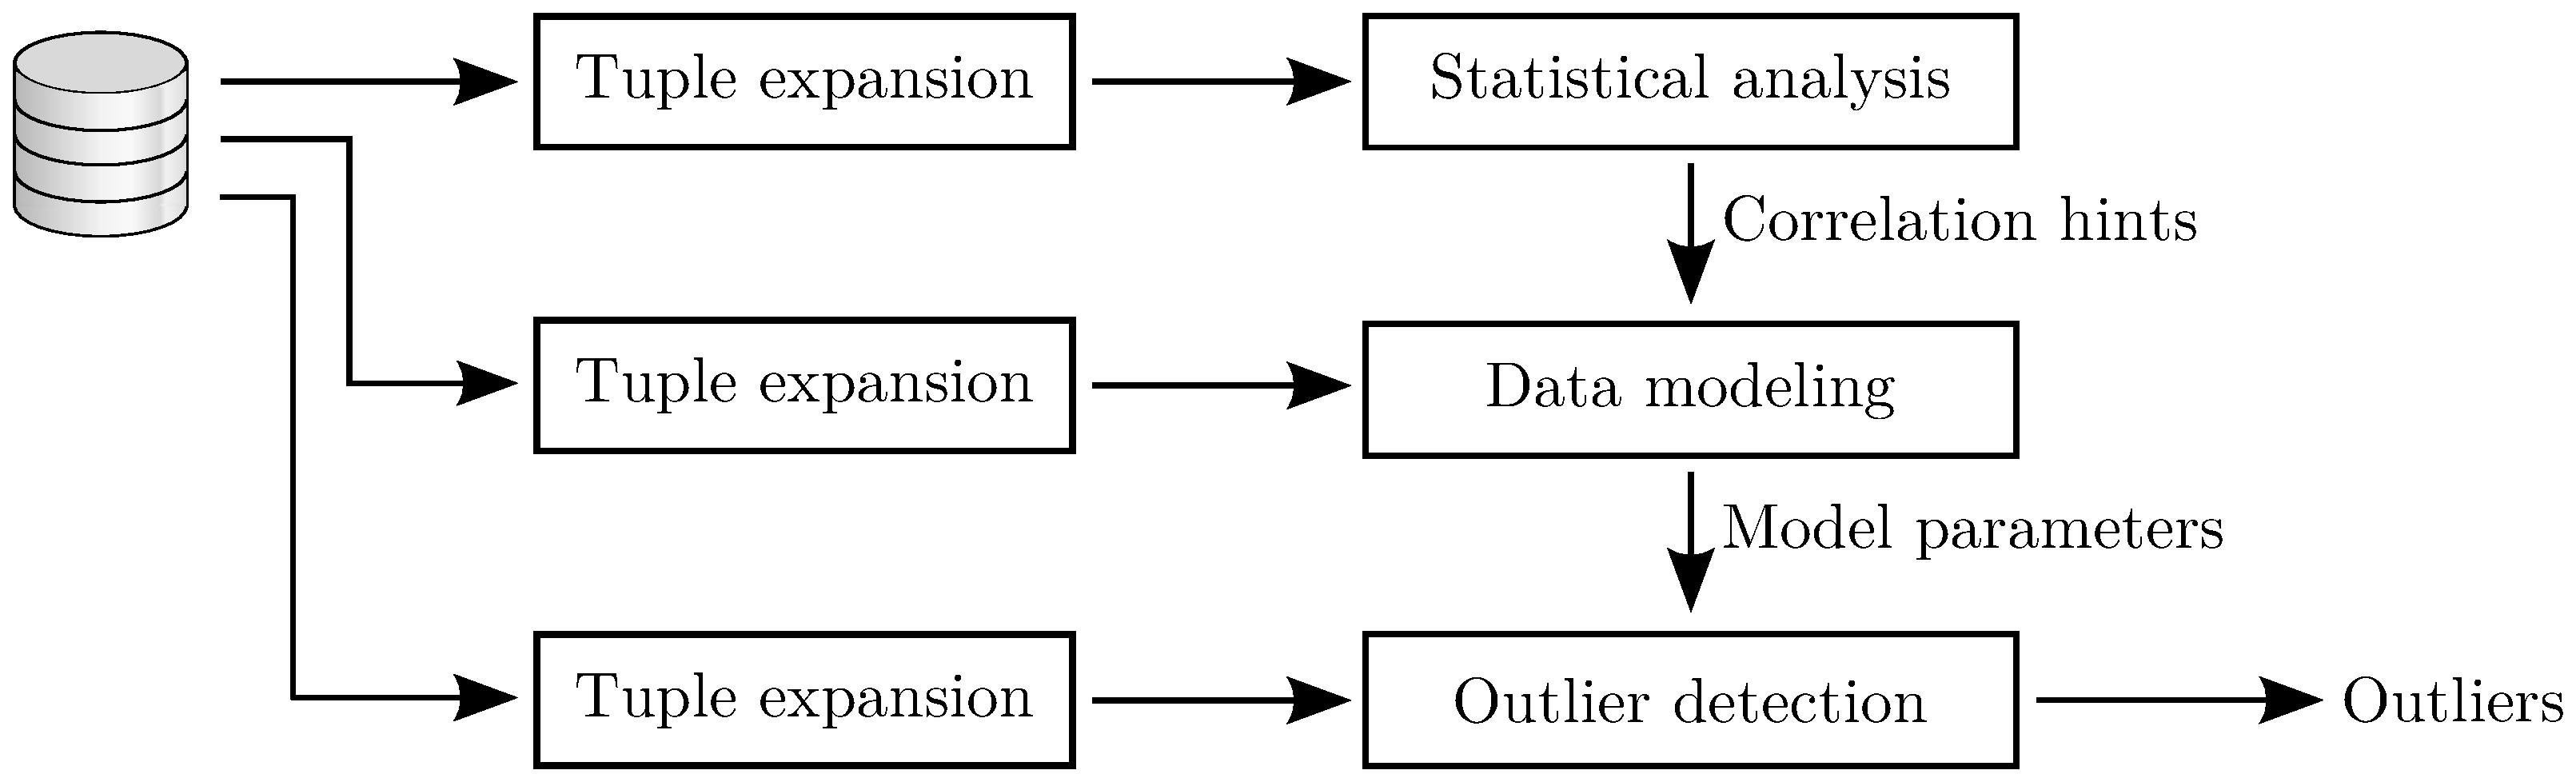
\includegraphics[width=\linewidth]{../graphics/pipeline.pdf}
        \end{figure}
      \end{block} \vspace{\blocksep}

      \vspace{-\baselineskip}
      \begin{columns}[t,totalwidth=\textwidth]
        \begin{column}{\colwidth}
          \newcommand{\picturecolumn}[2][1]{
    \begin{column}{.32\textwidth}
      \begin{figure}
        \centering
        \includegraphics[height=.75\linewidth,page=#1]{#2}
      \end{figure}
    \end{column}
}
\newcommand{\hsepline}{
  \par\vspace{-.75\baselineskip}
  \rule{0.9\linewidth}{1pt}
}

\begin{block}{\thighlight{Outliers characterization and detection}}
  \subttl{Statistical analysis}
  \begin{center}
    \begin{minipage}{.5\textwidth}
      \centering
      Pearson's correlation
      \hsepline{}
      Soft dependencies between numerical series
    \end{minipage}
  \end{center}
  
  \vspace{0.5\baselineskip}\subttl{Data modeling}
  \begin{columns}[T]
    \begin{column}{.32\textwidth}
      \centering
      Gaussian Model
      \hsepline{}
      Simple numerical data
    \end{column}
    
    \begin{column}{.32\textwidth}
      \centering
      Mixture Model
      \hsepline{}
      Multivariate numerical data
    \end{column}

    \begin{column}{.32\textwidth}
      \centering
      Histogram
      \hsepline{}
      Multivariate heterogeneous data
    \end{column}
  \end{columns}
  ~
  
  \subttl{Outlier Analysis}	
  \begin{columns}[T]
    \picturecolumn[1]{../graphics/models-plots-crop.pdf}
    \picturecolumn[2]{../graphics/models-plots-crop.pdf}
    \picturecolumn[3]{../graphics/models-plots-crop.pdf}
  \end{columns}
\end{block}
 \vspace{\blocksep}
        \end{column}

        \begin{column}{\colwidth}
          \section{Evaluation}
\label{sec:evaluation}

%\srm{Can we compare to some kind of ``baseline'' -- i.e., how well would these statistical methods do without access to expanded data?}

We implemented \dBoost/ as a library that runs on top of a standard relational database or set of structured data files. Our code is publicly available on GitHub under version 3 of the GNU Public License\footnote{\url{https://github.com/cpitclaudel/dBoost}}. The program is made of two parts: a library, and a number of data acquisition front-ends (CSV and SQL are currently supported). The library provides functions for each of the phases previously described, and includes a collection of expansion rules from Section~\ref{sec:expansion}.

%Table~\ref{table:flags} shows the usage options to run the models supported by \dBoost/. \fxnote{Should we keep this table? ** Add an appendix if we have room}

%\begin{table*}
%  \renewcommand{\arraystretch}{1.2}
%  \setlength\tabcolsep{3\tabcolsep}
%
%  \label{table:flags}
%  \caption{\dBoost/ command line usage.}
%  \centering
%  \begin{tabular} { l | l | p{10cm} }
%    \multicolumn{3}{l}{} \\
%    \hline
%    Flag & Options & Explanation \\
%    \hline
%    --gaussian & n\_stdev & Report outliers that fall more than n\_stdev standard deviations away from the mean of the data \\
%    --mixture & n\_subpops & Use a model of \texttt{n\_subpops} Gaussians \\
%         & threshold & Report outliers above threshold percentile \\
%    --histogram & peak\_s & Consider only fields with a peaked distribution with peakiness peak\_s \\
%         & outlier\_s & Report values that fall in classes with less than outlier\_s percent \\
%    --statistical & epsilon & Give hints to the model for correlations with Pearson $R$ coefficient greater than epsilon \\
%  \end{tabular}
%\end{table*}

This section presents the results of running our tool on the following real and synthetic datasets.

\begin{itemize}
\item \emph{Synthetic datasets}\\
  \textbf{Fizz-Buzz} A mixed textual-numerical dataset in which each record contains two entries: a number, and either ``Fizz'' if the number is divisible by 3, ``Buzz'' if the number is divisible by 5, ``FizzBuzz'' if it is divisible by both, and the number itself (as a string) otherwise. Outliers appear when the second column does not respect these rules; this can be a misplaced ``Fizz'', a missing ``Buzz'', or even a totally different string (e.g. ``Woof!'').\\
  \textbf{Web logins} A series of three non-numeric datasets in which entries contain the login time and connection location for different users. Each user has different connection habits, leading to different types of outliers.
\item \emph{Real-world datasets}\\
  \textbf{CSAIL Directory} A publicly-accessible directory of researchers\fxnote{Should we anonymize this?}, in which each record may include a first and a last name, a phone number, an office number, an email, and a job title. Outliers are hard to define mathematically in this case, and we instead demonstrate how the ideas exposed in previous sections of the paper come together to allow for efficient detection of unusual values.\\
  \textbf{Intel lab data} A publicly-available numerical dataset of temperature, light, humidity and voltage measurements. Outliers are due mostly to sensor glitches.
\end{itemize}

These datasets showcase the power of our methods, both in terms of classification power and expressiveness and succinctness when adding new rules to the system\footnote{Indeed, the set of rules used for tuple expansion is user-configurable, and new rules can be easily added; thus, specific knowledge about the data can be taught to the system by users, expressing some soft form of data integrity constraints.}. Where relevant we include performance measurements. These numbers intend to demonstrate that our approach is computationally reasonable and that our models scale linearly given a fixed training size. We show in Section~\ref{sec:performance-evaluation} how our prototype requires on the order of a few minutes to process a million elements using a high-level single-threaded scripting language. A production-ready implementation would run one or two orders of magnitude faster by taking advantage of the inherent parallelizability of the models, using an efficient on-disk representation of the data, and relying on a lower-level language with an efficient optimizing compiler.

The following subsections describe each of the test sets and associated results in greater detail.

\subsection{Soft constraint specifications: Fizz-Buzz}
We start with an extremely simple example, highlighting how easy our system makes it to encode and check data integrity constraints. The Fizz-Buzz programming exercise is based on a children's game and frequently found in programming interviews. The synthetic dataset we generated obeys the following rules: for each record \(x, y\), $x$ is a number between 0 and 1000, and $y$ is ``Fizz'' if \(x \mod 3 = 0\), ``Buzz'' if \(x \mod 5 = 0\), ``FizzBuzz'' if \(x \mod 15 = 0\), and \(x\) otherwise. In our synthetic dataset we introduced three outliers: \texttt{(25, "Fizz")}, \texttt{(28, "Woof!")}, \texttt{(30, "Buzz")}. Each demonstrates a different error, namely swapping ``Fizz'' and ``Buzz'', producing entirely incorrect output, and failing to recognize that a number is divisible by both $3$ and $5$.

A traditional way of checking that all tuples verify the production rule outlined above is to encode this rule itself as a database integrity constraint. This requires encoding the full complexity of the exercise in the rule, and would require manual adjustments if the rules were to change. Instead, a user might want to specify the bare minimum for the system to infer the rules; in this case, it is sufficient to add one extraction rule, mapping integers to two booleans denoting whether they are divisible by $3$ or $5$. Such a rule could be written like this:

\begin{minted}{python3}
@rule
def fizzbuzz(x: int) -> ("div 3", "div 5"):
  return (x % 3 == 0, x % 5 == 0)
\end{minted}

Running the discrete statistical analyzer on the synthetic datasets suggests that the two columns are correlated, and using the histogram model flags the aforementioned outliers. The output of the program for the \texttt{(30, "Buzz")} line, for example, is similar to:

\begin{lstnobreak}[gobble=2]
   $30$ $Buzz$
   > Values ($30$, '$Buzz$') do not
     match features ('$div 3$', '$strip numbers$')
   • histogram for ('div 3', 'strip numbers'):
     [532] ████████████████████ (False, '<num>')
     [133] █████ (False, 'Buzz')
     [  1] ▌ (False, 'Fizz')
     [  1] ▌ (False, 'Woof!')
     [  1] /▌/ $(True, 'Buzz')$
     [267] ██████████ (True, 'Fizz')
     [ 66] ██ (True, 'FizzBuzz')
\end{lstnobreak}

Using the partitioned histogram model produces similar output:

\begin{lstnobreak}[gobble=2]
   $30$ $Buzz$
   > Values ($30$, '$Buzz$') do not
     match features ('$div 3$', '$strip numbers$')
   • histogram for ('strip numbers',) if 'div 3' = True:
     [  1] /▌/ $('Buzz',)$
     [267] ████████████████████ ('Fizz',)
     [ 66] ████ ('FizzBuzz',)
   ... if 'div 3' = False:
     [532] ████████████████████ ('<num>',)
     [133] █████ ('Buzz',)
     [  1] ▌ ('Fizz',)
     [  1] ▌ ('Woof!',)
\end{lstnobreak}

\subsection{Logins: a more realistic partitioned dataset}

Our web activity synthetic datasets are comprised of two columns: a Unix timestamp stored as an \texttt{INT}, and a country. Each dataset is supposed to track the connections of a registered user on a website; such a dataset could be obtained by selecting the relevant rows out of a large table listing all connections of all users. Each user exhibits a different connection pattern:

\begin{itemize}
\item One user always connects from the same country; values that do not match this country are outliers.
\item The second connects from one country during the week, and from another during the week-end; outliers in this case are connections from a country that doesn't match the country for that day of the week.
\item The third user connects from a set of three countries, with no discernible pattern. This should not return any outliers.
\end{itemize}

The datasets are randomly generated sets of 2000 connections, listed in no particular order. The target outlier rate is \SI{5}{\percent} in each generated dataset.

\newcommand{\prop}[2]{#1\,\#\,#2}

As in the \emph{Fizz-Buzz} example, numerical models are useless here, whereas histogram-based models produce good results. In the first case, a histogram-based model with no correlation analysis is sufficient to flag the outliers (\timing{.08}{.14}{.38})\footnote{All runtime results were obtained using a 4 core i7-4810MQ CPU @ 2.80GHz and 32GB of RAM.}. In the second case, the discrete statistical analysis phase singles out interesting pairs of correlated columns, including \texttt{(\prop{date}{day of week}, country)} and \texttt{(\prop{date}{is weekend}, country)}. A histogram-based model is sufficient to successfully flag outliers, without resorting to partitioning.

\fxnote{Exclude self-correlations from the discrete analyzer to speed it up and get better results}

Mixing data from two or more users, however, shows the limits of the non-partitioned histogram approach. If we only look at two-columns correlations the individual behavior patterns become less apparent, and if we look at three-column correlations the histograms become too large and spurious hits start to appear due to the many discrete correlations hints returned by the analyzer. The partitioned histograms model, on the other hand, can handle the three-users without particular difficulties, by highlighting (among others) the triplet \texttt{(user, \prop{date}{is weekend}, country)} (\timing {.14}{.19}{.56}).
\subsection{CSAIL Directory}
\label{sec:csail-directory-evaluation}

The CSAIL directory is an online directory of about 1000 faculty, staff and students in the MIT Computer Science and Artificial Intelligence Laboratory\footnote{\url{https://www.csail.mit.edu/peoplesearch}}. Each entry contains a person's name, phone number, office number, email address, and position.

Some entries, such as a phone number, may be missing from the directory. Nonetheless, we expect our framework to be useful in flagging discrepancies between different records. Since the notion of what constitutes an outlier here is imprecise at best, we also expect the tool to allow the user to explore different sets of parameters. To illustrate the process, we present the results returned by two iterations of the tool in the next subsection, each with increasingly strict limits on the number of outliers returned. Because the CSAIL test set is exclusively textual, we use the histogram model for evaluation; continuous models would not fare as well, since only part of the expanded tuples are numeric.
We also manually annotated the dataset for outliers to determine the accuracy of our system.

\subsubsection{Initial run: low specificity filtering}
The search for outliers is initiated with parameters $\theta = 0.8, \epsilon = 0.2$ (\timing {0.36}{.11}{0.60}). Correlation detection is disabled for these experiments.

This invocation produces a long list of outliers; a small subset of these is presented below. For privacy reasons, names,  phone numbers, office numbers, and emails have been omitted or anonymized in the following listings.

\begin{figure*}
\centering
  \paddedgraphics{../../graphics/csail-stats}
  \caption{Accuracy of \dBoost/ on the CSAIL dataset, evaluated by comparison to manual annotation of outliers in the directory. Outliers were detected using $\theta = 0.8$ and $\epsilon = 0.025$; the tuples are sorted according to why they are -- or are flagged as -- outliers. The false positives in the last category are due to names whose proper capitalization is not title case. Green represents region of agreement between the output of \dBoost/ and manual annotation, red shows outliers in the manual annotation that \dBoost/ did not find, orange shows records that \dBoost/ flagged as outliers that the manual annotation did not, and grey indicates values that could not manually be categorized with complete certainty as either outlying or non-outlying.}

  \label{fig:csail-evaluation}
\end{figure*}

\begin{lstlisting}[gobble=2]
  Hacker, Alyssa, 32-D968,
    $aph@CSAIL.MIT.EDU$, Postdoctoral Associate
  > Value '$aph@CSAIL.MIT.EDU$' doesn't match feature '$lower case$'

  Bitdiddle, Ben, $NE47-989$,
    bbitdid@mit.edu, Graduate Student
  > Value '$NE47-989$' doesn't match feature '$signature$'

  $Lu-ater$, Eva, 32-G972,
    eva@csail.mit.edu, Research Scientist
  > Value '$Lu-ater$' doesn't match feature '$title case$'

  Tweakit, $ $, 32-G699,
    twktem@mit.edu, Administrative Assistant
  > Value '$ $' doesn't match feature '$empty$'
\end{lstlisting}

In total, 451 entries contain outliers, out of a total of 1000. Office numbers are often flagged, as well as names and email addresses. By changing the input parameters to $\theta = 0.8, \epsilon = 0.05$, most of the outliers due to office numbers disappear due to the lower sensitivity. \lstinline{Hacker, Alyssa} disappears from the list, since e-mails with inconsistent capitalization occur frequently enough in the database that they are not considered outliers at sensitivity level $\epsilon = 0.05$. After tuning these parameters, we are left with 68 outliers.

In addition to identifying outliers, \dBoost/ is equipped with tools that provide the user with additional feedback on why features were identified as outliers.

\begin{lstlisting}[gobble=2]
  Bitdiddle, Ben, $NE47-989$,
    bbitdid@csail.mit.edu, Graduate Student
   > Value '$NE47-223$' doesn't match feature '$signature$'
   • histogram for ('signature',):
     [266] ██████████ <empty>
     [  1] /▌/ $Lu,Lu,Nd,Nd,Pd,Nd,Nd,Nd$
     [  1] ▌ Lu,Nd,Nd,Pd,Nd,Nd,Nd
     [  2] ▌ Nd,Nd,Lu,Pd,Nd,Nd,Nd
     [485] ████████████████████ Nd,Nd,Pd,Lu,Nd,Nd,Nd
     [ 51] ██ Nd,Nd,Pd,Lu,Nd,Nd,Nd,Lu
     [155] ██████ Nd,Nd,Pd,Nd,Nd,Nd
     [ 36] █ Nd,Nd,Pd,Nd,Nd,Nd,Lu
     [  3] ▌ Nd,Nd,Pd,Nd,Nd,Nd,Nd
     [  1] ▌ Nd,Pd,Nd,Nd,Nd

  $Lu-ater$, Eva, 32-G972,
    eva@csail.mit.edu, Research Scientist
  > Value '$Lu-ater$' doesn't match feature '$title case$'
  • histogram for ('$title case$',):
    [ 15] /▌/ $False$
    [986] ████████████████████ True

  Tweakit, $ $, 32-G699,
    twktem@mit.edu, Administrative Assistant ...
  > Value '$ $' doesn't match feature '$empty$'
  • histogram for ('empty',):
    [1000] ████████████████████ False
    [   1] /▌/ $True$
\end{lstlisting}

Our tool highlights the incorrect field, and prints the corresponding histogram. The bin in which the suspicious value falls is also highlighted. The \texttt{signature} case is particularly interesting: recall that to extract the signature of a string, our tools replace each character by the name of its Unicode class; hence the string \texttt{NE47-989} is converted to \lstinline{Lu,Lu,Nd,Nd,Pd,Nd,Nd,Nd} (two letters, two numbers, one dash, three numbers), which does not fall in any of the dominant bins (the most frequent case, \lstinline{Nd,Nd,Pd,Lu,Nd,Nd,Nd}, describes office numbers like \lstinline{32-G804}, the predominant form of office numbering in the Stata Center).

Manual inspection of the results reveal that most of the outliers reported are actually bad inputs. There are, however, a number of false positives, such as:

\begin{lstlisting}[gobble=2]
  $DeFect$, Cy, 32-D597,
    cydf@csail.mit.edu, Graduate Student
  > Value '$DeFect$' doesn't match feature '$title case$'
  • histogram for ('$title case$',):
    [ 15] /▌/ $False$
    [986] ████████████████████ True
\end{lstlisting}

The case of \lstinline{DeFect} is correct, but our tool notes that it does not adhere to the casing standard derived from other tuples, and thus reports it.

We compared \dBoost/'s output to a manually annotated version of the CSAIL directory to analyze its accuracy; the results are shown in Figure~\ref{fig:csail-evaluation}.

\subsection{Intel Lab Data}
\label{sec:intel-lab-data-evaluation}

We also evaluated our outlier detection framework on sensor data from the publicly available Intel Lab Data set\footnote{\url{http://db.csail.mit.edu/labdata/labdata.html}}. The Intel Lab Data contains data collected from 54 sensors spread throughout the Intel Berkeley Research Lab. Each data entry contains information including temperature, humidity, light and voltage taken from a Mica2Dot sensor and weatherboard. The dataset contains a total of approximately 2.3 million measurements.

The Intel lab dataset has known outliers from faulty sensor readings due to periods of critically low voltage. During these periods, the sensors go haywire and produce faulty measurements. For example, the temperature may be registered as over $120$ degrees Celsius, which is obviously abnormal behavior in a human environment such as where the sensors were deployed.
 
We analyzed a sample of 1000 data points selected at random from the sensor data; due to the numerical nature of this data, the Simple Gaussian and Mixture models are better-suited to analyzing it than the Histogram model.

We also compare the results of our models to Local Outlier Factors, a common outlier detection methodology, in this section.
 
\subsubsection{Simple Gaussian Model}

The results from running the sensor data set through the Simple Gaussian model are shown in Figure~\ref{fig:gauss15}. The data is plotted in light green, and the outliers are marked by dark red crosses. 

In this experiment we flag the entries with column values that fall outside $1.5$ standard deviations of the mean of that particular column as outliers. This model runs relatively fast, as no correlations are computed (\timing{.03}{0}{.12}).
%As we observe in Figure~\ref{fig:gauss15}, this leads to the extreme values on the temperature spectrum as well as the humidity spectrum to be identified as outliers.
%However, many points in the normal range of operation are flagged as outliers.
%The cause of the noise can be seen in Figure~\ref{fig:sensors_gaus_1-5b}.
%In this plot we see that the values of both voltage and light are relatively evenly distributed within their respective ranges.
%Therefore many values lie outside $1.5$ standard deviations from the mean, despite having reasonable values in other dimensions such as temperature.
%Using information from correlations is one way in which we improve on this, which we describe in the next section.


\subsubsection{Mixture Model}
We set the statistical threshold to $0.7$, which produces two correlations between temperature and humidity and between temperature and voltage. 
Figure~\ref{fig:gmm1t1} shows the results when using a single Gaussian component. Points flagged as outliers have a likelihood of less than $7.5\%$ of being produced by the Gaussian generated by the model (\timing {.03}{.34}{.73}).

This model is able to detect values with high temperature and low voltage as outliers.
 
%We show in Figure~\ref{fig:sensors_nocorr} the benefits of pruning the data via correlations before feeding it into the Gaussian model.
%In this experiment, we allow the statistical analyzer to mark all columns as correlated.
%The model produces a Gaussian with so much noise from the light data that it detects many points even within the normal operating range as outliers, even when the threshold is reduced to $0.5\%$. 
%Thus, using some mechanism to find correlations is useful in narrowing the search space for outliers.
 
Figure~\ref{fig:gmm2t05} shows the results obtained using the Mixture model with two components, using the same 1000 randomly selected data points. Flagged values have a likelihood of less than $7.5\%$ under their dominant Gaussian (\timing {.03}{.35}{0.78}).
When using two Gaussians, the points clustered around the temperature $120$ degrees Celsius are no longer detected as outliers: they are modeled by their own Gaussian (although this Gaussian's weight is smaller than its counterpart). This model highlights the points within normal sensor operation that have outlying results.


\subsubsection{Local Outlier Factors}
\label{sec:lof-evaluation}

In this section we compare the results of our Gaussian and Mixture models to Local Outlier Factors (LOF)~\cite{Breunig2000}, a frequently used method for outlier detection.
LOF measures the degree to which a data point is an outlier by comparing each data point's reachability to those of its $k$ nearest neighbors.
The higher the LOF, the more isolated the data point relative to its local neighborhood and therefore the more likely the point is to be an outlier.

One downside of LOF compared to \dBoost/ is that it can only evaluate two-dimensional data.
The original algorithm also has significant computation complexity in order to calculate the distance to the nearest neighbors of each data point.
One benefit of LOF, however, is that the algorithm returns a continuous value that indicates the degree to which a point is an outlier, as opposed to a binary value.

Figure~\ref{fig:lofk2} shows the outliers detected by LOF when $k=2$.
We observe that contrary to the Gaussian and Mixture models, the outliers detected by LOF are scattered throughout the data.
The outliers are not necessarily the points one would intuitively assume are outliers.
This is because points that are within the normal range of the data will be selected as outliers if they are far enough away from the other points nearest to them.
%When the number of nearest neighbors evaluated is increased to $10$ in Figure~\ref{fig:lof_10}, the outliers detected are further outside the main cluster of points.
We find that LOF is not as useful at pointing out the tagged outliers in the sensor data set.



\subsection{Scalability}
\label{sec:performance-evaluation}

%We show in Figure~\ref{fig:scaling} how \dBoost/ scales as the amount of data used to build the models and to test on the models increases.
We measure the total runtime of our system, including the data modeling and outlier detection phases for the Simple Gaussian, Mixtures with 2 Gaussians, and Histograms. 
We used the Intel sensor data set from Section~\ref{sec:intel-lab-data-evaluation} to evaulate the Gaussian and Mixture models, and the CSAIL directory from Section~\ref{sec:csail-directory-evaluation} to evaluate the Histograms. 
We use random sampling to provide training sets of 1 thousand and 10 thousand elements from the Intel dataset to build the data models.
We test them on all 2+ million elements in the dataset.
To provide a more comprehensive study of the scalability of the Histogram model, we replicated the rows of the CSAIL directory to increase the training and test set sizes. 

In Figure~\ref{fig:scaling}, we show the runtime of our prototype. Each line shows a model trained with a different training set size. As shown in the figure, runtime scales linearly as the test set size increases.
Applying additional optimizations such as using a lower-level language or enabling parallism would improve runtime performance to production-ready levels. 

\begin{figure}
\centering
%\paddedgraphics{../graphics/scalability.pdf}
\caption{The scalability of the Gaussian and Mixture Models produced with different training sample sizes (listed next to the model in the legend) as the test set size increases.}
\label{fig:scaling}
\end{figure}

%\subsection{Presidential Campaign Finance}
\label{sec:presidential-campaign-evaluation}
\cite{PresCampaignData}

%\subsection{Mimic2}
\label{sec:mimic2-evaluation}

 \vspace{\blocksep}
          % \section{Future Work}
% \label{sec:future-work}
 \vspace{\blocksep}
        \end{column}      
      \end{columns}
    \end{column}      
  \end{columns}
\end{frame}
\end{document}